\input{header}

\AtBeginSubsection[]
{
	\begin{frame}<beamer>
		\frametitle{Outline}
		\tableofcontents[current,currentsubsection]
	\end{frame}
}

\begin{document}
\begin{frame}[allowframebreaks] \frametitle{Computability theory vs. complexity theory}
    \begin{itemize}
\item In Chapter 3 we showed that various TMs are equivalent
\item For example, single-tape and multi-tape TMs are equivalent
\item However, their ``time complexities'' are different
\end{itemize}\end{frame}

\begin{frame}[allowframebreaks] \frametitle{Complexity of Multi-tape
  TM}
  \begin{itemize}
  \item Theorem 7.8
    
  \item [] Let $t(n) \geq n$. For a $t(n)$ multi-tape TM

$\Rightarrow \exists$ equivalent 
$O(t(n)^2)$ single-tape TM
\item Idea for the proof: similar to how we proved their equivalence

\item We will show that simulating each step of a multi-tape TM
takes
$O(t(n))$ on a single-tape TM

\item Let $k$ be the number of tapes
\item How did we simulate a multi-tape TM?

  \begin{center}
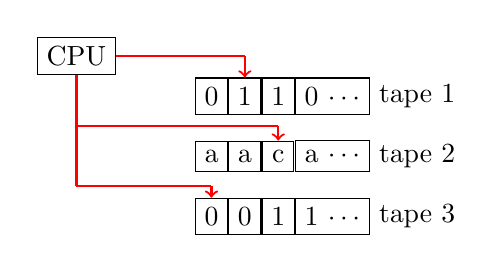
\begin{tikzpicture}[ampersand replacement=\&]
\matrix 
{
  \node[draw](0) {CPU}; \& [1cm]  \& \node(1){} ; \&\&\& \\
  \& \node[draw]{0}; \& \node[draw](a){1}; \& \node[draw]{1}; \& \node[draw]{0 $\cdots$};  \& \node{tape 1};\\
\node(2){} ; \&  \&  \& \node(21){} ; \&\& \\  
\& \node[draw]{a}; \& \node[draw]{a}; \& \node[draw](b){c}; \& \node[draw]{a $\cdots$}; \&  \node{tape 2}; \\
\node(3){} ; \& \node(31){} ; \&  \&  \&\& \\
\& \node[draw](c){0}; \& \node[draw]{0}; \& \node[draw]{1}; \& \node[draw]{1 $\cdots$}; \&  \node{tape 3}; \\
};

\draw [-,red,thick] (0) -- (1.center) ;
\draw [->,red,thick] (1.center) -- (a) ;
\draw [-,red,thick] (0) -- (2.center) ;
\draw [-,red,thick] (2.center) -- (21.center) ;
\draw [->,red,thick] (21.center) -- (b) ;
\draw [-,red,thick] (0) -- (3.center) ;
\draw [-,red,thick] (3.center) -- (31.center) ;
\draw [->,red,thick] (31.center) -- (c) ;
\end{tikzpicture}
\end{center}


\begin{center}
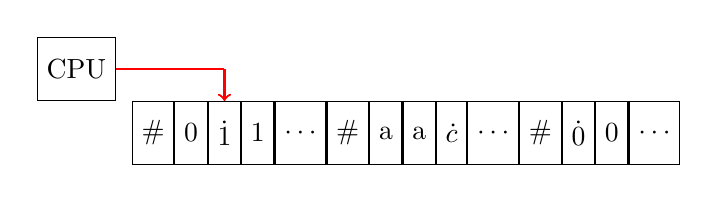
\begin{tikzpicture}[ampersand replacement=\&]
\matrix[nodes={minimum height=8mm}] 
{
  \node[draw](0) {CPU}; \& [0.2cm] \& \& \node(1){} ; \& \&\&\& \&\&\& \&\&\& \\
\& \node[draw]{\#};  \& \node[draw]{0}; \& \node[draw](a){$\dot{1}$}; \& \node[draw]{1}; \& \node[draw]{$\cdots$};
\& \node[draw]{\#};  \& \node[draw]{a}; \& \node[draw]{a}; \& \node[draw]{$\dot{\text{c}}$}; \& \node[draw]{$\cdots$}; 
\& \node[draw]{\#};  \& \node[draw](c){$\dot{0}$}; \& \node[draw]{0}; \& \node[draw]{$\cdots$}; \\
};

\draw [-,red,thick] (0) -- (1.center) ;
\draw [->,red,thick] (1.center) -- (a) ;
\end{tikzpicture}
\end{center}


\item To simulate each step of multi-tape TM, we scan to know where heads point to
  and do the update
\item However, we may have to
right shift the tape 
\item So we need to know the tape length. It is
\begin{equation*}
  k \times O(t(n)) = O(t(n)) 
\end{equation*}
  
\item Note that each tape of multi-tape TM has $O(t(n))$ length. Why?

\item A $t(n)$ multi-tape TM generates
$O(t(n))$ contents in 
$O(t(n))$ time

\item Thus the cost of
  simulating each step of multi-tape TM on a single-tape TM is
  $O(t(n))$
\item There are $O(t(n))$ multi-tape TM steps, so
  the total cost is
  \begin{equation*}
    O(t(n)) \times O(t(n)) = O(t(n)^2)
\end{equation*}
\end{itemize}\end{frame}

\end{document}
